\chapter{Introduction}
\label{ch:Introduction}

\section{General}

\subsection{Parkinson's Disease}

According to Patients Medical \cite{patients_medical_definition_2014}, \begin{quote}``Parkinson's disease is a progressive, neurodegenerative disease that occurs when the neurons within the brain responsible for producing the chemical dopamine become impaired or die. Dopamine is essential for the smooth control and coordination of the movement of voluntary muscle groups. Once approximately 80\% of the brain's dopamine producing cells no longer function, the symptoms of Parkinson's disease begin to appear. [\dots] Parkinson's disease may be termed as a progressive movement disorder that is distinguished by marked slow movements, tremors, and unstable posture.''\end{quote}

Especially in advanced stages of the Parkinson's disease (PD)\nomenclature{PD}{Parkinson's disease} many patients exhibit an episodic, brief inability to step that delays gait initiation or interrupts ongoing gait. This phenomenon is called freezing of gait and is often associated with an alternating shaking of the knees, called knee trembling. However, these clinical signs of balance or gait problems are not evident in early stages of the disease \cite{mancini_anticipatory_2009}\cite{jacobs_knee_2009}.

\subsection{Anticipatory Postural Adjustments}

A major challange to the human ballance control system is the fact that we are bipeds having only one foot in contact with the ground while walking, and that two-thirds  of our body mass is located two-thirds of body height above the ground \cite{halliday_initiation_1998}. Thus, to induce stable gait anticipatory postural adjustments (APAs)\nomenclature{APAs}{Anticipatory Postural Adjustments} are necessary. The Encyclopedia of Neuroscience \cite[p.133]{woollacott_anticipatory_2009} defines APAs as "A predictive motor response that acts to counter, in a preemptive manner, the postural destabilization associated with a forthcoming movement." As seen in Figure \ref{fig:APAoverview} the centre of body mass (COM)\nomenclature{COM}{Centre of Mass} is accelerated forward and laterally over the stance foot to make sure that the body does not fall laterally toward the stepping foot during the swing phase \cite{woollacott_anticipatory_2009}. The curve of the centre of pressure (COP)\nomenclature{COP}{Centre of Pressure} is divided in three periods. First, in the S1 period the COP moves posteriorly and toward the intended stepping limb, while the deliberate uncoupling of the COP and COM generates forward momentum. Then, in the S2 period, the COP displaces mediolaterally toward the stance foot. Finally, during the S3 period the COP moves anteriorly under the stance foot \cite{hass_gait_2005-1}.

\begin{figure}
	\centering
	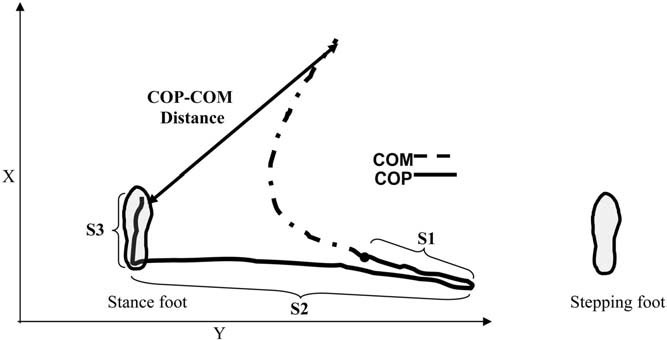
\epsfig{file=images/APA_overview, width=9cm}
	\caption{Representative anticipatory postural adjustments during forward-oriented gait initiation when stepping with the right foot. \cite{hass_gait_2005-1}.}
	\label{fig:APAoverview}
\end{figure}


\section{Goals}

The goal of the project was to analyse anticipatory postural adjustments prior to step inition and subsequently build a classifier using MATLAB, which is fed with data from both a force plate and a magnetic inertial measurement unit (GaitWatch \cite{olivares_vicente_gaitwatch_2013}) in order to distinguish between Parkinson patients and healthy subjects. To gather the data the subject stood in front of the force plate. Then, the GaitWatch and force plate record was started and the subject made a step onto the force plate. After standing upright for a variable time of two to ten seconds the subject left the force plate, made a few steps, turned left, and stopped in front of it again. This sequence was repeated ten times.


\section{Motivation}

Advanced PD can increasingly diminish quality of life, since patients are dependent on help from others to accomplish daily tasks. New neuroprotective medications are currently being developed and are expected to decelerate or stop the progression of the disease in early stages prior to significant loss of neurons \cite{botzel_motivation_2014}\cite{mancini_isway:_2012}. Thus, a quantitative PD classification, enabling early diagnosis of the disease, could optimise early treatment and could furthermore help to validate new treatment methods. Additionally, an objective evaluation of longterm treatment success was ensured.


\section{State of the Art}

There are several rating scales as well as technical equipment that has been used to assess Parkinson's disease and to analyse anticipatory postural adjustments.  They differ in terms of practicability, accuracy, validity, portability, and cost. The state of the art at the beginning of the project is described below.

\subsection{Rating Scales}

A commonly used rating scale is the Unified Parkinson’s Disease Rating Scale (UPDRS),\nomenclature{UPDRS}{Unified Parkinson’s Disease Rating Scale} which is a short test performed by a physician \cite{klerk_long-term_2009}. The patient is rated on 31 different items (see Table \ref{tab:UPDRS}) with a score of 0 (normal) to 4 (severely affected) \cite{herndon_handbook_2006}. Another method is the rough, but widely utilised and accepted Hoehn and Yahr scale (HY)\nomenclature{HY}{Hoehn and Yahr scale}. Parkinsonian motor impairment is categorised in 5 stages: Unilateral (Stage 1) to bilateral disease (Stage 2) without balance difficulties, to the presence of postural instability (Stage 3), loss of physical independence (Stage 4), up to being wheelchair- or bed-bound (Stage 5) \cite{goetz_movement_2004}. Finally, there is the Timed Up and Go Test (TUG)\nomenclature{TUG}{Timed Up and Go Test}. This clinical test consists of rising from a chair, walking three metres, turning, walking back, and sitting. The total duration then represents the clinical outcome. It is widely used to rate balance, mobility, and fall risk in PD in its entirety, but does not give information about the particular impairements \cite{palmerini_quantification_2013}.

Without the need for complex technical devices these tests are relatively simple to perform. \citeauthor{klerk_long-term_2009} \cite{klerk_long-term_2009} mentioned their disadvantages, including subjectivity, short observation periods, and unfamiliarity of the environment that these rating methods bring along. Further limitations are caused by clinician's bias and insensitivity to mild impairments (floor effect) \cite{mancini_isway:_2012}.

\begin{table}[h]
\begin{tabular}{lll}
\hline
Mentation, mood & Activities of daily & Motor examination \\
and behavior & living & \\
\hline
Intellectual impairment & Speech & Speech \\

Thought disorder & Salivation & Facial expression\\

Depression & Swallowing & Tremor at rest \\

Motivation/initiative & Handwriting & Action or postural tremor of hands \\

& Use of eating utensils & Rigidity \\

& Dressing & Finger taps\\

& Hygiene & Hand movements\\

& Turning in bed & Rapid alternating movements of hands\\

& Falling & Food agility\\

& Freezing when walking & Arising from chair \\

& Walking & Posture\\

& Tremor & Gait\\

& Sensory Complaints & Posture stability\\

& & Body bradikinesia and hypokinesia \\
\hline
\end{tabular}
\caption{Unified Parkinson's Disease Rating Scale items adapted from \cite{herndon_handbook_2006}.}
\label{tab:UPDRS}
\end{table}

\subsection{Instrumentation}

In addition to the aforementioned subjective rating scales, there are different devices used to quantify gait and posture to assess them objectively. All of them come with certain pros and cons. The following devices have been used:

\subsubsection{Electromyographs} Electromyography is a technique for evaluating the electrical activity of skeletal muscles. Successive action potentials generated by muscle cells are measured, by means of needle electrodes inserted into the muscles, and displayed on a cathode-ray oscilloscope. Thus medical abnormalities can be detected. The instrument used to capture the visual recording, termed electromyogram, is called electromyograph \cite{encyclopedia_britannica_electromyography_2014}. Electromyography is constrained to clinical application only, but in return gives indication about the contribution of specific, individual muscles to APAs.

\subsubsection{Force Plates} Force plates quantify the ground reaction force (GRF)\nomenclature{GRF}{Ground Reaction Force}, that is, the force exerted to the human body by the ground. The GRF is a three-dimensional vector with three orthogonal components. One component along the direction of gravity, one parallel to the ground in the sagittal plane, and one parallel to the ground in the frontal plane. Those are vertical planes that divide the body in left and right halves, and ventral and dorsal sections, respectively. A force plate usually gives an electrical voltage proportional to the force in each of the three directions. Force plates can be characterised according to the following criteria: Sensitivity in Volts per Newton, crosstalk (indication of vertical force if a horizontal force is applied and vice versa), repeatability (similar results under the same load), and time- and temperature drift \cite{griffiths_principles_2006}. Usually force plates are embedded in the ground to place minimum constraints on subjects \cite{mancini_trunk_2011}. Therefore they are limited to clinical application. They have the advantage that they don't need to be calibrated before each use. 

\subsubsection{Inertial Measurement Units} Devices that use a combination of inertial sensors like accelerometers and gyroscopes are referred to as inertial measurement units (IMUs)\nomenclature{IMU}{Inertial Measurement Unit}. If they also include magnetic field sensors (magnetometers), they are called magnetic inertial measurement units (MIMUs)\nomenclature{MIMU}{Magnetic Inertial Measurement Unit}. With these devices the orientation of the body can be obtained with up to nine degrees of freedom, provided that triaxial accelerometers and magnetometers are used, respectively \cite{olivares_vicente_signal_2013}.

\begin{itemize}

\item \textsc{Accelerometers} measure the acceleration of an object relative to an inertial frame. Since acceleration cannot be measured directly, the force exerted to a reference mass is obtained and the resultant acceleration is computed according to Newton's second law $ \mathbf{F} = m \cdot \mathbf a $ \cite{encyclopedia_britannica_accelerometer_2014}.

\item \textsc{Gyroscopes} measure angular velocity and are based on the Coriolis Effect. By means of integration of the angular velocity the rotation angle is obtained \cite{olivares_vicente_signal_2013}.

\item \textsc{Magnetometers} measure the strength and the direction of the magnetic field in a point in space, using the relationship between magnetic fields, movement and induced currents \cite{olivares_vicente_signal_2013}.
 
\end{itemize}
MIMUs are portable and relatively inexpensive. They can be easily attached to the body and thus allow non-clinical longterm application. Their drawbacks are complex calibration procedures and drift behaviour over time, depending on intensity and duration of the movement. Hence, in order to maintain a satisfactory degree of precision, periodical recomputation of the calibration parameters is required \cite{olivares_vicente_signal_2013}. Moreover, \citeauthor{mancini_isway:_2012} \cite{mancini_isway:_2012} pointed out the need of data pre-processing and the question of how to generate a clinically understandable presantation of the movement data.

\subsection{Classification}

There are several research works in the literature dealing with APA analysis and PD classification, as the examination of posture and gait are key components of the clinical evaluation of PD \cite{palmerini_classification_2013}.

\citeauthor{klerk_long-term_2009} \cite{klerk_long-term_2009} developed a measurement system called PD Monitor, implementing an Activity Classifier that quantifies tremor and bradykinesia in the arm, thigh, and trunk, in an ambulant way and over long periods of time. They validated their measurements with video records, which were rated by physicians using the UPDRS and concluded that ``the PD monitor can be used for a detailed evaluation of the PD motor symptoms in order to optimize treatment.'' \cite{klerk_long-term_2009}.

\citeauthor{mancini_anticipatory_2009} \cite{mancini_anticipatory_2009} found that the eleven untreated early-to-moderate stage Parkinson's patients that took part in their study have a significantly smaller peak COP displacement towards the stepping leg and peak trunk acceleration towards the stance leg compared to the twelve age-matched healthy control subjects. Even though step velocity and step length were not different. The results showed that lateral APAs are impaired in early, untreated PD and that they are detectable with inertial sensors. As well as force plate-based, also acceleration-based extracted features could be used to detect impairments equally well. Due to the fact that the acceleration signal can be easily obtained via a sensor on a belt, no matter if in clinical or home environment, APA detection by means of accelerometers is considered as a useful way to characterise patients in early stages of PD without evident clinical symptoms. Additionally in \cite{mancini_anticipatory_2009} it is proposed to carry out further studies to determine the relationship between small APAs and the probability to develop start hesitation and freezing.

\citeauthor{palmerini_classification_2013} \cite{palmerini_classification_2013} states that PD classfication could deliver a tool to follow the progression of the disease during the entire course to examine the efficiency of treatment. They studied classification of PD subjects  using triaxial accelerometers on the lower back at L5 level and an ad hoc wrapper feature selection technique designed in \cite{palmerini_quantification_2013}. Linear discriminant analysis was used to obtain a classifier that permits clinical interpretation of the results. Twenty early-mild PD subjects and twenty healthy age-matched control subjects had to perform two simple tests (quiet standing, Timed Up and Go test), in two evaluations over a one-year follow-up, to test accuracy and robustness over time. They achieved satisfactory accuracy of 93.75\% and considered feature selection to be essential in this kind of data set. As well as \cite{mancini_anticipatory_2009} they found that lateral dynamics i.e. range of motion are impaired in early-mild PD and suggested further investigation on validity of measures in later stages.

\citeauthor{hass_gait_2005-1} \cite{hass_gait_2005-1} investigated the magnitude of the separation between the centre of pressure and the centre of body mass during gait initiation and its correlation with the severity of PD. They observed that the peak COP-COM distance during the S3 period (see Figure \ref{fig:APAoverview}), of the 20 participating patients with H\&Y score of 2.5 or higher, was 16\% smaller than the one of the 23 patients with H\&Y score of 2.0 or less. The results showed that this approach can quantify impairment of balance in PD at various stages of the disease.

On 13th of August 2014, the Michael J. Fox Foundation for Parkinson’s Research (MJFF)\nomenclature{MJFF}{Michael J. Fox Foundation for Parkinson’s Research} and Intel Corporation \cite{Intel_2013} announced a collaborative research study on objective measurement of PD symptoms. They aim to collect movement data of thousands of patients twenty-four seven at over 300 samples per second by means of unobtrusive wearable devices and store them on a big data analytics platform. The data platform, deployed on a cloud infrastructure, supports an analytics application that processes the data and detects changes in real time. Thus, by detecting anomalies, the progression of the disease can be measured objectively without the need for scientists to focus on the underlying computing technologies. Physicians and researchers are intended to have access to the data as well as be able to submit their own anonymised patient data for analysis. According to \cite{Intel_2013} the correlation of data that quantifies symptoms such as slowless of movement, tremor, and sleep quality with molecular data could advance drug development and provide a deeper insight into the clinical course of PD. At the end of 2014 Intel and MJFF plan to launch a mobile application, with which patients can report medication intake and how they are feeling to permit medical researchers to assess the effects of medications on motor symptoms. The extraordinary large scale of this project makes it unique in research.

\citeauthor{khorasani_hmm_2014} \cite{khorasani_hmm_2014} compared a Hidden Markov Model (HMM)\nomenclature{HMM}{Hidden Markov Model} based classifier against a sophisticated nonlinear classifier. The raw gait data corresponding to sixteen healthy and fifteen PD subjects was preprocessed and the stride interval i.e. length of gait cycle served as the input for the HMM classifier. Their results showed that the HMM method can distinguish between healthy subjects and PD patients with an accuracy of 90.3\%, similar to the accuracy obtained with the least squares support vector machine (LS-SVM)\nomenclature{LS-SVM}{Least squares support vector machine} implemented in \cite{wu_statistical_2010}.

\citeauthor{mancini_isway:_2012} \cite{mancini_isway:_2012} found that untreated PD affects postural control, even if it is not clinically apparent. They measured the acceleration on the posterior trunk at L5 level of thirteen patients recently diagnosed with PD, but not taking anti-parkinsonian medications, and twelve healty, age-matched control subjects to quantify the active postural corrections. To assess the smoothness of postural sway they calculated the jerk, which is the time derivative of the acceleration. At the same time they measured the COP with a force plate and determined, in contrast to \cite{mancini_anticipatory_2009}, an increased magnitude of both COP and acceleration signal in subjects with untreated PD in comparison with the control subjects. On top of this both signals contained a larger jerk, i.e. showed faster components in the untreated PD subjects. They concluded that acceleration based parameters as well as COP parameters are able to distinguish between the two groups. 



\section{Document Structure}

